\subsection{Datamodel}
\label{subsection:Datamodel}
Een van de belangrijkste doelen van de afstudeeropdracht is om een nieuw datamodel te maken voor een CMS-systeem.
Dit datamodel moet veel verschillende soorten datastructuren kunnen ondersteunen en deze kunnen presenteren op een \gls{Beheerder} zijn website.
Het huidige CMS van Snakeware doet dit door middel van een complexe structuur.
Deze structuur zorgt ervoor dat het moeilijk is om nieuwe functionaliteit toe te voegen en dat het systeem lastig is te onderhouden.

\whitespace
Daarom heeft het nieuwe datamodel twee belangrijke uitgangspunten om de pijnpunten van het oude CMS te voorkomen.
Het datamodel moet generiek blijven, zodat er veel verschillende datastructuren in opgeslagen kunnen worden.
Door het datamodel generiek en flexibel te houden hoeft het systeem niet uitgebreid te worden om een nieuwe datastructuren te ondersteunen.
Verder moet de structuur van het datamodel simpel blijven, zodat het makkelijk te onderhouden is.
Om deze doelen te bereiken is er gebruikgemaakt van de volgende concepten.

\whitespace
\textbf{Fields}

\whitespace
Content op websites bestaan uit kleinere stukken data\slash content.
Fields representeren de kleinste laag content op een website. 
Hierbij kan gedacht worden aan een stukje tekst of een prijs op een pagina.
Om bij fields een beter beeld te schetsen is er een stuk van de Snakeware website (snakeware.com) gebruikt als voorbeeld.
In figuur \ref{fig:VisualisationFields} wordt weergegeven waar de fields zich bevinden in de content.

\whitespace[2]
\begin{graphic}
    \captionsetup{type=figure}
    \caption{Visualisatie van fields}
    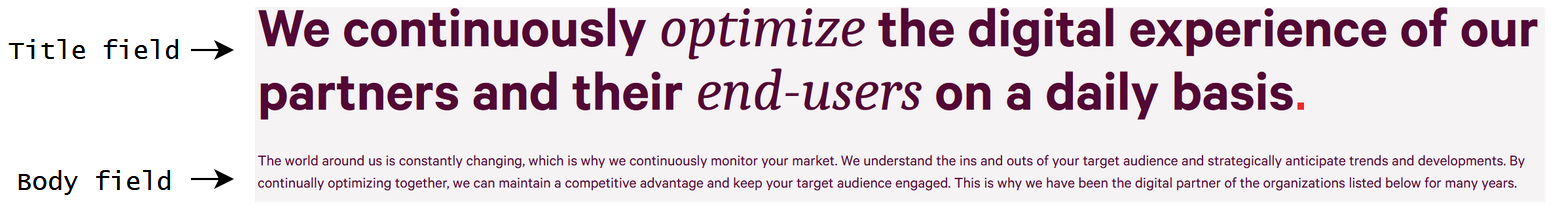
\includegraphics[scale=0.30]{VisualisationFields.png}
    \label{fig:VisualisationFields}
\end{graphic}

\whitespace
\textbf{Items}

\whitespace
Om een samenhangend stuk content op te stellen wordt er gebruikgemaakt van items.
Een item is een container dat meerdere fields kan bevatten.
Om hier een beter beeld bij te schetsen is hetzelfde voorbeeld gebruikt voor de items (zie figuur \ref{fig:VisualisationItems}).

\whitespace[2]
\begin{graphic}
    \captionsetup{type=figure}
    \caption{Visualisatie van een item}
    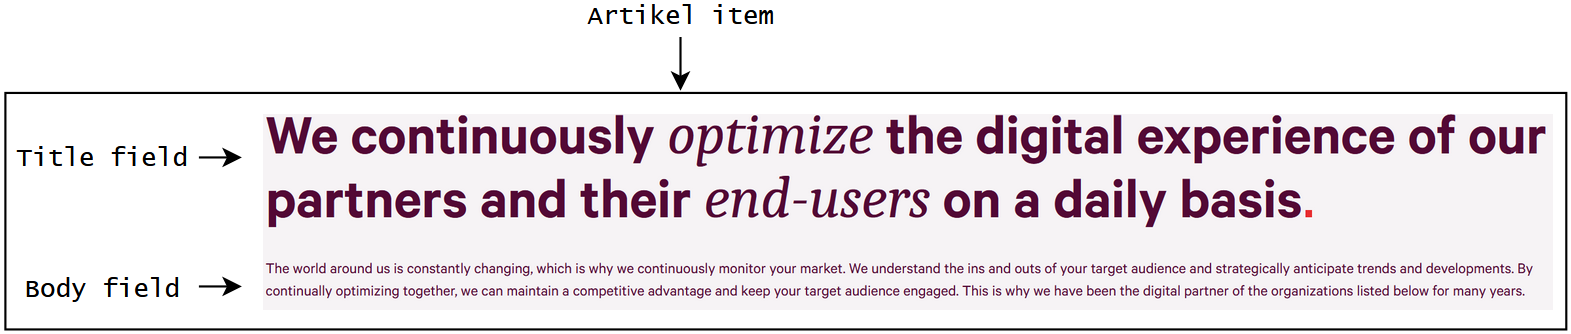
\includegraphics[scale=0.35]{VisualisationItems.png}
    \label{fig:VisualisationItems}
\end{graphic}

\whitespace
In het voorbeeld (figuur \ref{fig:VisualisationItems}) is te zien dat het item \qw{Artikel} 2 fields heeft.
Deze fields zijn \qw{Title} en \qw{Body} en bevatten de teksten voor de gedefinieerde gedeeltes van het item.
Een ander functionaliteit van een item is dat het meerdere items kan bevatten. 
Door dit te doen is het mogelijk om complexe structuren op te bouwen.

\whitespace
Om ervoor te zorgen dat items hergebruikt kunnen worden, wordt er gebruikgemaakt van templating.
Hierom zijn er item en field definities gemaakt die aangeven welke fields verplicht zijn op een item en welke optioneel.
In het ontwerp worden deze definities ItemDefinition en FieldDefinition genoemd.
Een klassendiagram met het geïntegreerde templating systeem is te zien in figuur \ref{fig:ClassDiagramItemFieldWithDefinition}.
Het datatype \qw{Content} bevat verschillende primaire types zoals integer, string, boolean ect.

\whitespace[2]
\begin{graphic}
    \captionsetup{type=figure}
    \caption{Klassendiagram datastructuur afstudeeropdracht}
    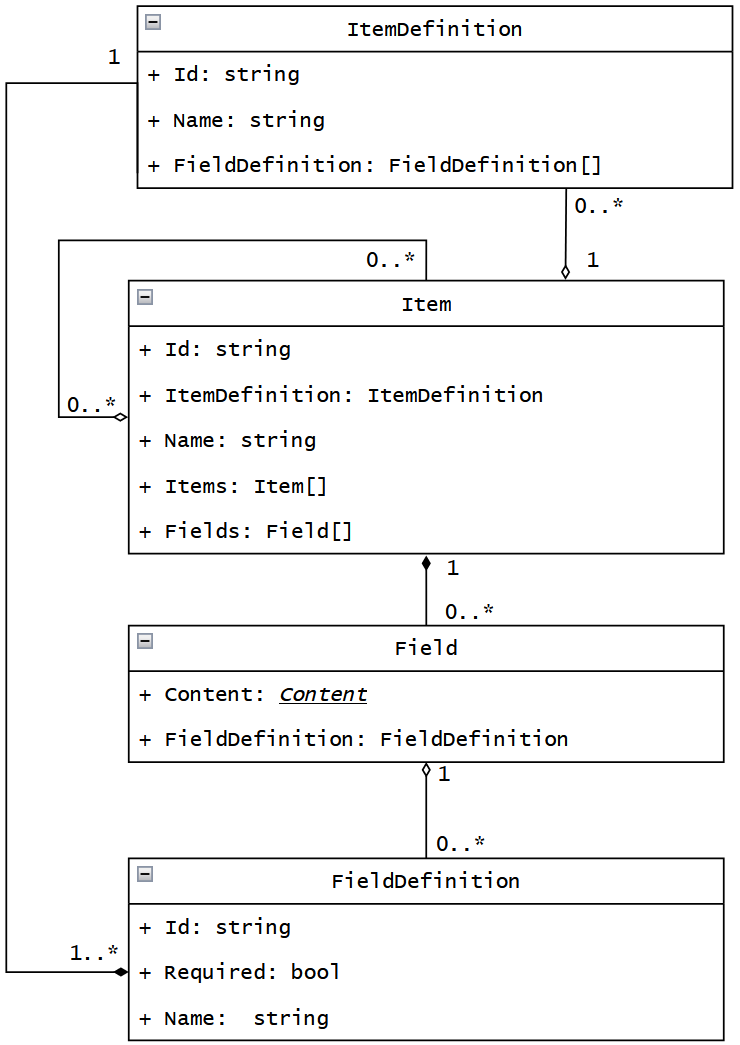
\includegraphics[scale=0.6]{ClassDiagramItemFieldWithDefinition.png}
    \label{fig:ClassDiagramItemFieldWithDefinition}
\end{graphic}

% \todo[inline]{Hier kloppen een paar relaties niet}
